%%%% PROCESAR con PdfLaTeX !!!!!


\documentclass[12pt]{book}
\usepackage{geometry}\geometry{top=2cm,bottom=2cm,left=3cm,right=3cm}
\usepackage{amssymb}
\usepackage{amsmath}
\usepackage{graphicx}
\usepackage{txfonts}




\begin{document}
\thispagestyle{empty}

\begin {center}

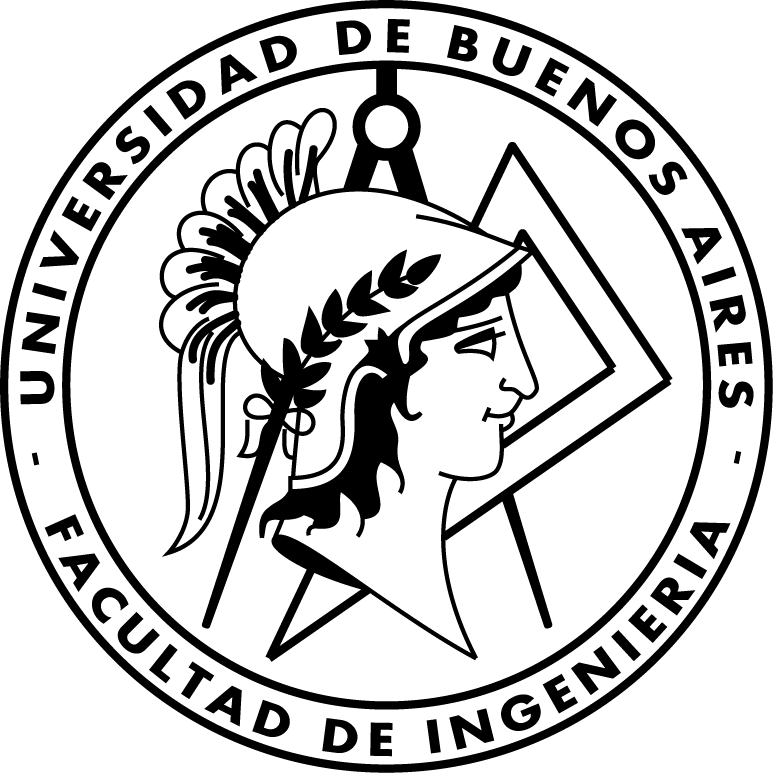
\includegraphics[scale=.4]{Logo-fiuba_big.png}

\medskip
UNIVERSIDAD DE BUENOS AIRES

Facultad de Ingenier\'ia

Departamento de Economia, Organizaci\'on y legal


\vspace{3cm}


\textbf{\large 7114 Modelos y Optimizaci\'on 1}

\vspace{2cm}


Este es un modesto aporte para los alumnos de la f\'acultad de ingenier\'ia  de la UBA de las carreras de licenciatura en an\'alsis de sistemas e ingenier\'ia inform\'atica.
De ninguna man\'era pretende ser una gu\'ia de estudio, ni remplaza las clases presenciales, el material oficial de la catedra esta disponible en el web site de la m\'ateria.
\\
wwww.ModelosUno.com.ar

\end {center}


\vspace{2.5cm}

\noindent Autor:	\,Isaac Edgar Camacho Ocampo
 
\noindent Carrera:	\,Licenciatura en An\'alisis de sistemas

\vspace{1cm}

\vspace{1cm}

\noindent Buenos Aires, 2019

\newpage

\tableofcontents

\chapter{Introducci\'on}La vida nos suele colocar, todo el tiempo, ante la disyuntiva de tener que elegir entre varios caminos. A veces esa libertad de decisión es una experiencia dramática, por las cosas que están en juego.

Es que cada elección trae aparejadas consecuencias, efectos que impactan en uno mismo y en otras personas. En la vida empresarial las decisiones clave descansan en quienes cumplen funciones gerenciales.

La contratación de empleados, la recisión de un contrato con el cliente más importante, la ampliación o remodelación de la línea de producción, la toma de un crédito, por ejemplo, pasa por ellos.

Pero también sobre los gerentes pesan determinaciones dramáticas, como el cierre de la empresa, el llamado a concurso de acreedores, o vender todo y empezar de nuevo.

Y como se sabe, toda decisión entraña un riesgo, porque existe la posibilidad de equivocarse. Es que nadie tiene garantías sobre el futuro, ya que lo que ocurra realmente puede desmentir todos los cálculos.

En este sentido, las decisiones gerenciales pueden llevar al éxito de la organización o a su fracaso. Si son acertadas, garantizan la sustentabilidad y el desarrollo si no, conducen al peor final.

Los expertos definen a la decisión como el resultado de un proceso mental-cognitivo de una persona o de un grupo de individuos. Se conoce como toma de decisiones al proceso que consiste en concretar la elección entre distintas alternativas.
\section{Investigación Operativa}
La Investigación Operativa es una disciplina moderna que utiliza modelos matemáticos, estadísticos y algoritmos para modelar y resolver problemas complejos, determinando la solución óptima y mejorando la toma de decisiones. Esta materia también recibe el nombre de Investigación de Operaciones, Investigación Operacional o Ciencias de la Administración.

Actualmente la Investigación Operativa incluye gran cantidad de ramas como la Programación Lineal, Programación No Lineal, Programación Dinámica, Simulación, Teoría de Colas, Teoría de Inventarios, Teoría de Grafos, etc.

\section{Definición aceptada por la SADIO}
La sociedad argentina de Investigación Operativa dice que \'esta es la aplicación de ciencia moderna a problemas complejosque aparecen en la dirección y administración de sistemas constituidos por hombres,
materiales, equipos y dinero en la industria, el comercio, el gobierno y la defensa. Su característica primordial es la elaboración de modelos científicos que mediante la incorporación de factores de riesgo e incertidumbre permitan evaluar decisiones, políticas y alternativas. Su objeto es auxiliar al directivo o al administrativo en la selección científica de susdecisiones.

\section{Mod\'elos}
\subsection{¿Que es modelizar?} Es hacer una simplificacion de la realidad y nosotros trabajamos con esa simplificacion ya que la realidad es muy compleja.
\subsection{¿Para que hacer un modelo?}
\begin{itemize}
\item \textbf{Economia de recursos:} Al igual que en la ingenieria civil cuando se hacen planos para representar una obra (ya que no seria l\'ogico hacer el edificio y ante un error rehacerlo), cuando modelamos un problema usando programacion lineal y dada la escazes de recursos, es mas eficiente trabajar sobre modelos.
\item \textbf{Eficiencia}: de nuevo so no tengo recursos limitantes entonces trabajo sobre la realidad y no modelo nada.
\item \textbf{simplicidad}: puedo mediante abstracci\'on lograr un modelo mas sencillo y eliminar la complejidad inherente del problema.
\item \textbf{En resumen es mejor que hacer multiples ensayos.}
\end{itemize}
Los mod\'elos se aplican a problemas de desici\'on y este existe cuando existen formas alternativas de actuar, con distintos resultados y diferentes eficiencias para lograr el objetivo es decir existen dudas respecto del curso alternativo a utilizar.


\section{Elementos de un modelo}
\subsection{Hipótesis y supuestos:} Para simplificar el modelo se delimita el sistema en estudio a través de las hipótesis y
supuestos simplificativos. Así se comienza a transformar el sistema físico en un modelo simbólico.
Las hipótesis deben ser probadas científicamente. Los supuestos son hipótesis que no pueden probarse.

\textbf{Ejemplos:}
Si estamos modelando una panaderia, y el recurso agua no es limitante y por otro no se dice nada de 				la venta de lo producido podemos agregar las hipotesis
\begin{enumerate}
	\item 	
	\textit{Hay agua suficiente para todos los procesos}
	\item
	\textit{Se vende todo lo que se produce}
\end{enumerate}
\subsection{Objetivo: }Mide la eficiencia de nuestro sistema y lo que buscamos es hallar la merjo solucion. El objetivo surge como respuesta a tres preguntas:
\\¿Qué hacer? es decir que es lo que queremos determinar.
\\¿Cuándo? (período de tiempo) puede ser un mes o año o un periodo t si no se especifica.
\\¿Para qué? para maximizar ganancias, o minimizar costos, nunca ambos a la vez.
\subsection{Actividad}
Proceso unitario que se realiza en el sistema físico caracterizado por consumir recursos
y/o generar un resultado económico y/o indicar un estado, por ejemplo producir un bien o indicar si se finaliz\'o un proceso.
\subsection{Variables}
Son las que miden o indican el estado de una actividad.
Las que miden pueden ser continuas o enteras.
Las que indican son, generalmente, variables (0,1) o bivalentes

\section{Programación lineal}La programación lineal es el campo de la programación matemática dedicado a maximizar o minimizar una función lineal, denominada función objetivo, de tal forma que las variables de dicha función estén sujetas a una serie de restricciones expresadas mediante un sistema de ecuaciones o inecuaciones también lineales.
\subsection{Programación Lineal Continua}
\subsection{Programación Lineal Entera}Es una tecnica que permite modelar y resolver problemas cuya caracterıstica principal
es que el conjunto de soluciones factibles es discreto.
\\
\\

\begin{itemize}
\item \textbf{OR l\'ogico}
\[ Y_{or} \quad \leq \quad \sum_{i=1}^{n}Y_{i} \quad \leq \quad n Y_{or}\]
\item \textbf{AND l\'ogico}
\[ n Y_{and} \quad \leq \quad \sum_{i=1}^{n}Y_{i} \quad \leq \quad (n-1) + Y_{and} \]
\end{itemize}


\subsection{Supuestos básicos de la Programación Lineal Continua}
\subsubsection{Proporcionalidad}
Tanto el beneficio como el uso de recursos son directamente proporcionales al nivel de
actividad
\subsubsection{Aditividad}No existen interacciones entre las actividades que cambien la medida total de la
efectividad o el uso total de algún recurso
\subsubsection{Divisibilidad}Las unidades de actividad pueden dividirse en niveles fraccionarios cualesquiera, de
modo que pueden permitirse valores no enteros para las variables
\subsubsection{Certeza}Todos los parámetros del modelo son constantes conocidas

\section{Centros de producción}
\subsection{Armado vs Mezcla}

\section{Conceptos previos}
\begin{enumerate}
	\item \textbf{Eficiencia:} Producir mas con menos recursos o productividad.
	\item \textbf{Eficacia:} Lograr el resultado aunque se consuman muchos recursos.
	\item \textbf{Costo de oportunidad:} Es el costo de producir una unidad de un bien.
	\item \textbf{Contribucion marginal:} Ganancia neta.
\end{enumerate}




\end{document}
